\begin{center}
    
\includegraphics[width=0.2\textwidth]{Сборы/Зимние сборы 2025/hearths.png}
\end{center}

\begin{flushright}
        \scriptsize{finally dude...}
\end{flushright}

\problem{1}
Докажите, что на изображенный на клетчатой бумаге треугольник $PQR$ является равнобедренным.

\centerline{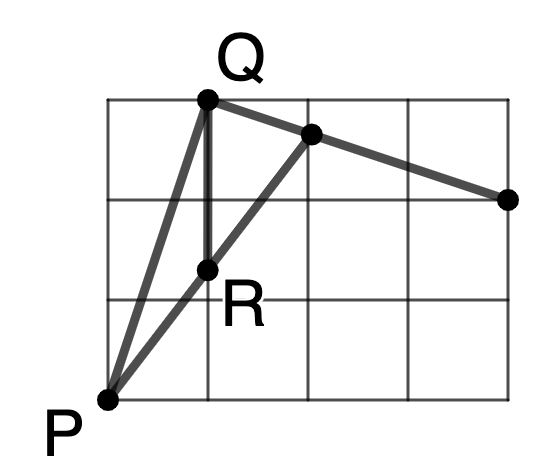
\includegraphics[width=0.3\linewidth]{Сборы/Зимние сборы 2025/6.png}}

\problem{2}
В треугольнике $ABC$ провели две биссектрисы угла $B$ - внутреннюю $BL$ и внешнюю $BK$. Найдите отношение $CK:CL$, если $AB=5$, $BC=3$.

\problem{3}
Докажите, что в треугольнике $ABC$, в котором провели биссектрису $BL$, выполняется соотношение $\frac{BI}{IL} = \frac{AB+BC}{AC}$, где $I$ - центр вписанной окружности.

\problem{4}
На сторонах $AB$ и $BC$ треугольника $ABC$ взяли такие точки $E$ и $K$, что $AE : BE = 1 : 4$, $BK : CK = 2 : 3$. В каком отношении медиана $BM$ треугольника $ABC$ делит отрезок $EK$?

\problem{5}
Две окружности пересекаются в точках $P$ и $Q$. На одной их них взята произвольная точка $M$. Прямые $MP$ и $MQ$ повторно пересекают вторую окружность в точках $A$ и $B$ соответственно. Докажите, что длина отрезка $AB$ не зависит от выбора точки $M$. 

\problem{6} В остроугольном треугольнике $ABC$ проведена медиана $BM$. Точки $P$ и $Q$ -- центры вписанных окружностей треугольников $ABM$ и $CBM$ соответственно. Докажите, что вторая точка пересечения описанных окружностей треугольников $ABP$ и $CBQ$ лежит на отрезке $BM$.

\problem{7} Вершина $C$ прямого угла треугольника $ABC$ лежит внутри окружности с центром $O$ и радиусом $R$, проходящей через концы гипотенузы $AB$, $CH$ -- высота треугольника $ABC$. На прямой $AB$ взята точка $K$ так, что $KH = OH$. Найдите $CK$.

\newpage

\begin{center}
    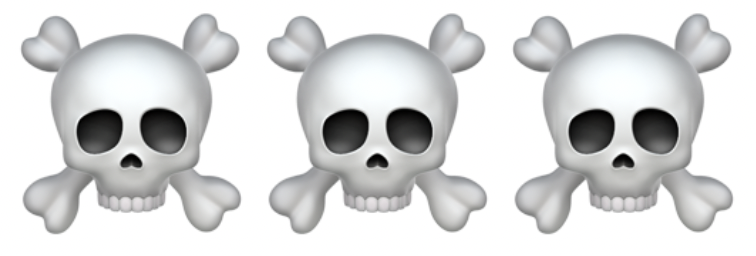
\includegraphics[width=0.2\textwidth]{Сборы/Зимние сборы 2025/skulls.png}
\end{center}

\begin{flushright}
        \scriptsize{nah bro u kidding me...}
\end{flushright}

\problem{1} 
Rectangles $B C C_1 B_2, C A A_1 C_2$, and $A B B_1 A_2$ are erected outside an acute triangle $A B C$. Suppose that

$$
\angle B C_1 C+\angle C A_1 A+\angle A B_1 B=180^{\circ}
$$


Prove that lines $B_1 C_2, C_1 A_2$, and $A_1 B_2$ are concurrent.

\problem{2}
Given a triangle $A B C$, let $P$ and $Q$ be points on segments $\overline{A B}$ and $\overline{A C}$, respectively, such that $A P=A Q$. Let $S$ and $R$ be distinct points on segment $\overline{B C}$ such that $S$ lies between $B$ and $R, \angle B P S=\angle P R S$, and $\angle C Q R=\angle Q S R$. Prove that $P, Q, R, S$ are concyclic (in other words, these four points lie on a circle).

\problem{3}
Let $A B C$ be an acute-angled triangle and let $D, E$, and $F$ be the feet of altitudes from $A, B$, and $C$ to sides $B C, C A$, and $A B$, respectively. Denote by $\omega_B$ and $\omega_C$ the incircles of triangles $B D F$ and $C D E$, and let these circles be tangent to segments $D F$ and $D E$ at $M$ and $N$, respectively. Let line $M N$ meet circles $\omega_B$ and $\omega_C$ again at $P \neq M$ and $Q \neq N$, respectively. Prove that $M P=N Q$.

\problem{4}
Triangle $A B C$ has circumcircle $\Omega$ and circumcenter $O$. A circle $\Gamma$ with center $A$ intersects the segment $B C$ at points $D$ and $E$, such that $B$, $D, E$, and $C$ are all different and lie on line $B C$ in this order. Let $F$ and $G$ be the points of intersection of $\Gamma$ and $\Omega$, such that $A, F, B, C$, and $G$ lie on $\Omega$ in this order. Let $K$ be the second point of intersection of the circumcircle of triangle $B D F$ and the segment $A B$. Let $L$ be the second point of intersection of the circumcircle of triangle $C G E$ and the segment $C A$.

Suppose that the lines $F K$ and $G L$ are different and intersect at the point $X$. Prove that $X$ lies on the line $A O$.

